\documentclass[11pt,a4paper,reqno]{amsart}
\usepackage{geometry}               % See geometry.pdf to learn the layout options. There are lots.
\usepackage[parfill]{parskip}       % Begin paragraphs with an empty line rather than an indent
\usepackage[table]{xcolor}          % xcolor with table
\usepackage{bm}                     % bold math
\usepackage{graphicx}               % include graphics
\usepackage[
    colorlinks=true,
    citecolor=black,
%    linkcolor=black,
    urlcolor=blue,
]{hyperref} % make references into hyperlinks

\geometry{left = 3cm, right = 3cm, top = 3cm, bottom = 3cm} % reduce margins
\frenchspacing                      % single space between sentences

\graphicspath{ {fig/} }

\title{Design and validation of a static bicycle simulator}
%\author{Oliver Lee}

% define common math terms
\newcommand{\mass}{\bm{M}}
\newcommand{\damping}{v \bm{C}_1}
\newcommand{\stiffness}{g \bm{K}_0 + v^2 \bm{K}_2}

% state terms
\newcommand{\dstate}{\dot{\bm{x}}}
\newcommand{\state}{\bm{x}}
\newcommand{\sysInput}{\bm{u}}
\newcommand{\sysOutput}{y}
\newcommand{\stateMat}{\bm{A}}
\newcommand{\inputMat}{\bm{B}}
\newcommand{\outputMat}{\bm{C}}

% estimate terms
\newcommand{\dstateEst}{\dot{\hat{\bm{x}}}}
\newcommand{\stateEst}{\hat{\bm{x}}}
\newcommand{\meas}{z}
\newcommand{\processCov}{\bm{Q}}
\newcommand{\processNoise}{\bm{w}}
\newcommand{\measCov}{R}
\newcommand{\measNoise}{v}
\newcommand{\kalmanGain}{\bm{K}}
\newcommand{\estimateCov}{\bm{P}}

% coordinates and speeds
\newcommand{\x}{x_{p}}
\newcommand{\y}{y_{p}}
\newcommand{\pitch}{\theta}
\newcommand{\yaw}{\psi}
\newcommand{\roll}{\phi}
\newcommand{\steer}{\delta}
\newcommand{\dx}{\dot{x}_{p}}
\newcommand{\dy}{\dot{y}_{p}}
\newcommand{\pitchRate}{\dot{\theta}}
\newcommand{\yawRate}{\dot{\psi}}
\newcommand{\rollRate}{\dot{\phi}}
\newcommand{\steerRate}{\dot{\phi}}

\begin{document}
\maketitle

\section{Introduction}
%% overview on cycling
%% address safety in cycling, understanding rider behavior
Cycling is a common form of transportation in a number of countries.
While cycling has long been prevalent as a low-cost form of transportation in many developing countries,
there has been a resurgence in ridership for developed countries including
the U.S.\cite{mckenzie2014}, the U.K.\cite{FIXME}, and throughout Europe\cite{FIXME}.
%road traffic estimates in Great Britain, 2014
A large proportion of non-fatal injuries to cyclists result from single bicycle crashes,
with the proportion ranging from 60\% to 95\% for a number of countries in Europe\cite{schepers2014}.
%As these do not involve other vehicles, the cause of these accidents can be limited to bicycle handing qualities and
%environmental factors.
A better understanding of the bicycle rider system is beneficial in understanding these accidents and is necessary to
reduce these in number and to improve the safety of cyclists.

%% history on bicycle and rider research
% FIXME: references used in 'Data collected for ..'
The bicycle has been used for transport since the 19th century\cite{wilson2004}, but the body of work studying this
vehicle is smaller relative to motorized vehicles such as motorcycles, cars, and planes.
Whipple first developed a general model for the bicycle in 1899\cite{whipple1899}.
A multitude of others have contributed to bicycle research; Meijaard presents a detailed history on bicycle dynamics and
notes many of the seminal figures, along with verification of the correctness of the Whipple model\cite{meijaard2007}.
Kooijman shows some experimental validation of this (uncontrolled) model within the predicted stable speed
range\cite{kooijman2008}.
%% FIXME: bicycle research history
Models, as well as real world experience, show the bicycle rider system to be unstable for a range of speeds;
active control from the rider is required rider to stabilize the bicycle.
Recent work in the field of bicycle dynamics has focused on identification of rider control
models by means of experimental data collection\cite{delange2011,hess2012,hladun2015}.
Data collected for lateral line tracking\cite{delange2011,hess2012}, lane change\cite{hladun2015}, and stabilization
with roll torque disturbances\cite{delange2011,hess2012} were used for system identification and parameter estimation of
the gains of the human controller.

%% why is a simulator important (motivation for building a simulator)?
% goal of system identification
In car driver behavior research, studies have commonly used driving simulators\cite{steen2011}.
System identification has been used to evaluate performance-based driver steering models designed to match real driver
behavior\cite{pilutti1999,steen2011}.
To a smaller extent, this has also been done with motorcycle simulators for studying rider behavior\cite{kovacsova2015}.
There are always limitations with simulators;
certainly with a static simulator, one is incapable of simulating the vestibular inputs.
Studies from Crundall using static simulators suggest vestibular sensory input may not be necessary for system
identification of motorcycle riders\cite{crundall2012}.
Additionally, rider lean control has been shown to be ineffective relative to steer control\cite{sharp2008}
and experiments have shown very little upper body lean relative to the bicycle rear assembly when observing
riders\cite{kooijman2009}.

However, a simulator with high enough fidelity provides a number of benefits compared to using instrumented bicycles.
Namely, reproducibility of experiments, ease of data collection, and improved safety in test environments
come from use of simulators over instrumented vehicles /in real-world environments\cite{dewinter2012}.
As the rider bicycle system is unstable, simulators allow for tests of scenarios that have high risk of injury if
instrumented bicycles were to be used.

There have been a number of groups that have developed bicycle simulators for a variety of research goals.
The Korean Advanced Institute of Science and Technology has developed a pair of networked bicycle simulators to simulate
racing environments\cite{kwon2002}.
The simulators are built on a Stewart platforms and include steering and pedaling subsystems.
The bicycle dynamics assume that the mass of the frame and handlebar are evenly distributed between the front and rear
wheels.
Yin and He also describe the design of a simulator mounted on a Stewart platform with steering and pedaling
subsystems\cite{he2005, yin2007implementation} which is sued to study rider-bicycle models\cite{yin2007study}.
Additionally, the virtual environment is displayed using 3 projectors to create an immersive environment.
The bicycle dynamics are an implementation of the equations derived by Hand\cite{hand1988}.
Input torques are estimated from the measured acceleration of the respective coordinate.
Other bicycle simulators have been developed to study cognitive processes and focus less on realistic modeling of
bicycle dynamics.
FIVIS simulator is also designed using an entire bicycle mounted on a Stewart platform and similarly uses multiple
projectors to create an immersive visual environment\cite{herpers2008}.
It is used for safety education and rider training.
Plumert describes a bicycle simulator used to study rider behavior and decision making in traffic\cite{plumert2004}
where an instrumented bicycle on rollers is used to determine motion in a virtual environment.
The study focuses on rider perception and accurate steering feel is not addressed.
Other research using this simulator also focuses on rider behavior and decision making in
traffic\cite{plumert2007,chihak2010,grechkin2013}.
Similarly, Caro uses an instrumented bicycle on rollers to drive a bicycle in a virtual environment to study rider's
speed perception\cite{caro2015}.
De Lange created a simulator in MATLAB with the rider controlling the virtual bicycle by means of a
gamepad\cite{delange2011}.
His simulator provides visual but not vestibular or proprioceptive feedback and de Lange determines it the
simulator is not useful for analyzing rider control due to difficulty in controlling the bicycle.
As a precursor to this work, Schwab and Recuero prototyped a simulator with actuated handlebars\cite{schwab2013},
presenting the rider with visual and proprioceptive feedback.
In a preliminary study with two participants, they find haptic handlebar feedback torque necessary for the rider to
stabilize the bicycle;
participants failed to stabilize the bicycle for more than a few seconds without feedback torque.

This work describes the design of a bicycle simulator that will be used for primarily for research in system
identification and human rider control.
That is, the simulator was designed to accurate simulate steering dynamics and forces generated due to the
bicycle-environment interface.
However, this does not preclude the simulator from use in rider behavior studies.

We begin with a description of the model used and, at a high-level, the software and hardware design of the simulator.
Then a test procedure to evaluate simulator fidelity is presented.
Simulator data and data from naturalistic studies are compared and discussed.
Finally, we end with some conclusions and suggestions for future work.

\section{Simulation of the bicycle equations of motion} \label{sec:sim_eom}
\subsection{Steer Dynamics} \label{sec:steer_dynamics}
\subsubsection{Whipple Linearized Model}

The simulator uses the Whipple model\cite{whipple1899} along with a benchmark set of parameters generated by
Meijaard\cite{meijaard2007}.
A table with the coordinates and parameters that describe the model are provided in
\autoref{tab:coordinates} and \autoref{tab:parameters} and depicted in figures TODO \autoref{fig:bicycle}.
The model describes the equations of motion in terms of rear assembly roll angle $\roll$ and relative front and rear
assembly steer angle $\steer$, linearized about the nominal, or zero roll and zero steer, configuration
\begin{equation}
    \mass \ddot{\bm{q}} + \damping \dot{\bm{q}} + (\stiffness) \bm{q} = \bm{f} \label{eq:eom}
\end{equation}
where
$ \bm{q} = \begin{bmatrix} \roll & \steer \end{bmatrix}^T $,
$ \dot{\bm{q}} = \begin{bmatrix} \rollRate & \steerRate \end{bmatrix}^T $,
$ \ddot{\bm{q}} = \begin{bmatrix} \ddot{\roll} & \ddot{\steer} \end{bmatrix}^T $,
$ \bm{f} = \begin{bmatrix} T_\roll & T_\steer \end{bmatrix}^T $ with $ T_\roll $ and $ T_\steer$ the input roll
torque and steer torque of the system.
$ \mass $ is the mass, $ \damping $ the damping, and $ \stiffness $ the stiffness of the system,
parameterized by forward velocity $ v $ and $ g $ is gravitational acceleration.

This model assumes an idealized contact between the bicycle tires and ground, no-slip knife-edge point contact,
and the rider is rigidly fixed to the bicycle rear assembly.
The rider can apply a steer torque $ T_\steer $ but is unable to apply a roll torque $ T_\roll $ as there is no means to
do so.
There are no environmental factors that contribute a roll torque (such as crosswind) and as such,
we always take $ T_\roll = 0 $ and can rewrite the input as $ \bm{f} = \begin{bmatrix} 0  & T_\steer \end{bmatrix}^T $.
While the rider arms are necessary to provide the input steer torque $ T_\steer $, the movement of the arms is
neglected in this model.

% TODO: While Jason does mention these things in his PhD dissertation, perhaps it is better to cite another paper?
Torque sensors are commonly used to provide input to the simulated equations of motion\cite{FIXME}; the torques
necessary to steer a bicycle are small with magnitudes commonly between 0 and 3 Nm\cite{moore2012}.
While sensors that can accurately measure torques in this range do exist, any measurements may suffer from large
cross-torques induced by the rider in directions orthogonal to the steer axis.
In these cases, others have designed ways to obtain an accurate measurement of steer torque\cite{moore2012}.
However, given that a high resolution encoder measures steer angle, we numerically compute the steer
angular acceleration $ \ddot{\steer} $ in order to estimate the rider applied steer torque $ T_\steer $.

The dynamics of the physical handlebars are described by the following equation of motion
\begin{equation}
    I_\steer \ddot{\steer} = T_\steer- T_f \label{eq:handlebar_eom}
\end{equation}
where $ I_\steer $ is the moment of inertia of the handlebar about the steer axis and $ T_f $ the feedback torque
applied to the handlebars.

\subsubsection{State Estimation}
The roll angle $ \roll $ is simulated and presented to the rider via the visual environment.
Obtaining the roll angle $ \roll $ requires the plant to be observable which can be ascertained by evaluating the rank of
the observability matrix
\begin{equation}
    \bm{\mathcal{O}} = \begin{bmatrix} \outputMat \\ \outputMat\stateMat \\
                                       \outputMat\stateMat^2 \\ \outputMat\stateMat^3 \end{bmatrix}
\end{equation}
where $ \bm{A} $ and $ \bm{C} $ are the state and output matrices of the state space form of \autoref{eq:eom}.
We measure only steer angle $ \steer $ and have the resultant state space equations
\begin{equation}
\begin{aligned}
    \dstate &= \stateMat \state + \inputMat \sysInput \\
    \sysOutput &= \outputMat \state \label{eq:ss}
\end{aligned}
\end{equation}
where $ \dot{\bm{x}} = \begin{bmatrix} \rollRate & \steerRate & \ddot{\roll} & \ddot{\steer} \end{bmatrix}^T $,
$ \bm{x} = \begin{bmatrix} \roll & \steer& \rollRate & \steerRate \end{bmatrix}^T $,
and $ \bm{u} = \bm{f} $ from \autoref{eq:eom}.
The state space matrices are defined as
\begin{equation}
\begin{aligned}
    \stateMat &= \begin{bmatrix} \bm{0} & \bm{I} \\
                -\mass^{-1} (\stiffness) & -\mass^{-1} (\damping) \end{bmatrix} \\
    \inputMat &= \begin{bmatrix} \bm{0} \\ \mass^{-1} \end{bmatrix} \\
    \outputMat &= \begin{bmatrix} 0 & 1 & 0 & 0 \end{bmatrix}
\end{aligned}
\end{equation}
Note that the system is still parameterized by forward speed $ v $  as can be seen by the expression for
state matrix $ \stateMat $.

We find the observability matrix $ \bm{\mathcal{O}} $ to be full rank for all forward speeds except
$ v_1 = FIXME $ and $ v_2 = FIXME $.
The system is not observable at these velocities, however we limit the precision of the forward speed $ v $ in the
simulation to maintain an observable system.

TODO: compute observability matrix for speeds and generate plots


As the system is observable, we estimate the unmeasured states with a Kalman filter.
For this system, roll angle $ \roll $ and roll rate $ \rollRate $ do not exist in the physical setup and can only be
obtained through estimation.
While it is possible to obtain the steer rate $ \steerRate $ through a direct measurement with an angular rate
gyroscope, the bandwidth trade-off from estimation is minimal (TODO: compute and show this).
Given the system equations in \autoref{eq:ss}, we describe the Kalman filter model as the state space equations with
process and measurement noise
\begin{equation}
\begin{aligned}
    \dstateEst &= \stateMat \stateEst + \inputMat \sysInput + \processNoise \\
    \meas &= \outputMat \stateEst + \measNoise \label{eq:kalman_ss}
\end{aligned}
\end{equation}
where $ \stateEst $ and $ \dstateEst $ denote the state estimate and time derivative of the state estimate,
$ \processNoise $ and $ \measNoise $ are realizations of the process and measurement noise respectively,
and $ \meas $ is used to explicitly distinguish the system measurement from the system output $ \sysOutput $.

Process noise $ \processNoise $ and measurement noise $ \measNoise $ are drawn from random processes with
Gaussian distributions and described by the
process noise covariance matrix $ \processCov $ and measurement noise covariance matrix $ \measCov $.
% TODO: mention that Q > 0 and R >= 0?
The noise covariance matrices are assumed constant when the system has reached steady-state
(i.e. $ v $ is not changing with time). % what about steady turning?
As a result, we obtain the optimal Kalman gain matrix $ \kalmanGain $
%and estimate covariance matrix $ \estimateCov $
parameterized by forward speed $ v $, as well as system state estimate $ \stateEst $.

\subsection{Kinematics}

In modeling, a number of coordinates used to describe the kinematics of the bicycle are independent of the stability, or
steer dynamics as described in \autoref{sec:steer_dynamics}.
These \textit{ignorable} coordinates include
rear wheel contact point coordinates $ x_p $ , $ y_p $,
rear frame pitch angle $ \pitch $, and rear frame yaw angle $ \yaw $.
The kinematics of the bicycle are described with the following equations for the rear wheel contact $ (\x, \y) $ and
yaw angle $ \yaw $ as calculated by Meijaard\cite{meijaard2007}
\begin{equation}
\begin{aligned}
    \dx &= v \cos{\yaw} \\
    \dy &= v \sin{\yaw} \\
    \yawRate &= \frac{v \steer + c \steerRate}{w} \cos{\lambda} \label{eq:kineq}
\end{aligned}
\end{equation}
Refer to \autoref{tab:parameters} for a description of the model parameters.
Pitch angle $ \pitch $ is a dependent coordinate and the full nonlinear form cannot be expressed in a simple closed-form
expression.
A simpler approach is to compute analytic expressions for $ \pitch $, $ \pitchRate $ as constraints, and with the aid of
a computer algebra system (such as SymPy\cite{sympy}), and find the roots using an algorithm such as Newton-Raphson.
As the constraint derivative can be defined analytically, is continuous, and a good initial guess exists (i.e. the pitch
angle in the nominal configuration), we are guaranteed quadratic convergence.
An example to generate the analytic expressions for $ \pitch$ and $ \pitchRate $ is given
\href{https://github.com/oliverlee/bicycle/blob/master/python/pitch_constraint.py}{here}.
Note that changes of the pitch angle $ \pitch $ are small and the first order approximation is zero due to symmetry of
the bicycle model about the $ xz $-plane.

\section{Software implementation}
The simulation of the bicycle equations of motion as described in \autoref{sec:sim_eom} is implemented as three main
components:
\begin{itemize}
    \item visualization engine
    \item simulation engine
    \item hardware controller
\end{itemize}
The three components are separate in both software and hardware.
The simulation engine acts as a root node in the network topology and data is communicated over TCP/IP.
\subsection{Visualization}
The simulator visualization is built using \href{https://unity3d.com/}{Unity}, a cross-platform game engine used to
develop video games.
The Unity Editor is used to create a virtual environment and to define a basic description for the bicycle model;
an example of the virtual environment is provided in \autoref{fig:unity}.

The bicycle is composed of a hierarchy of basic shapes which are grouped into the rear wheel, rear frame, front frame,
and front wheel, as is done in the bicycle model.
Shape size is dependent on parameters used by the bicycle model and are transmitted at the start of the simulation.
Physics effects are disabled as the bicycle is modeled and simulated separately.
Upon receiving the bicycle coordinates, the translation of the $ xy $-contact point and relative rotations for each body
are set.

\begin{figure}
    \centering
    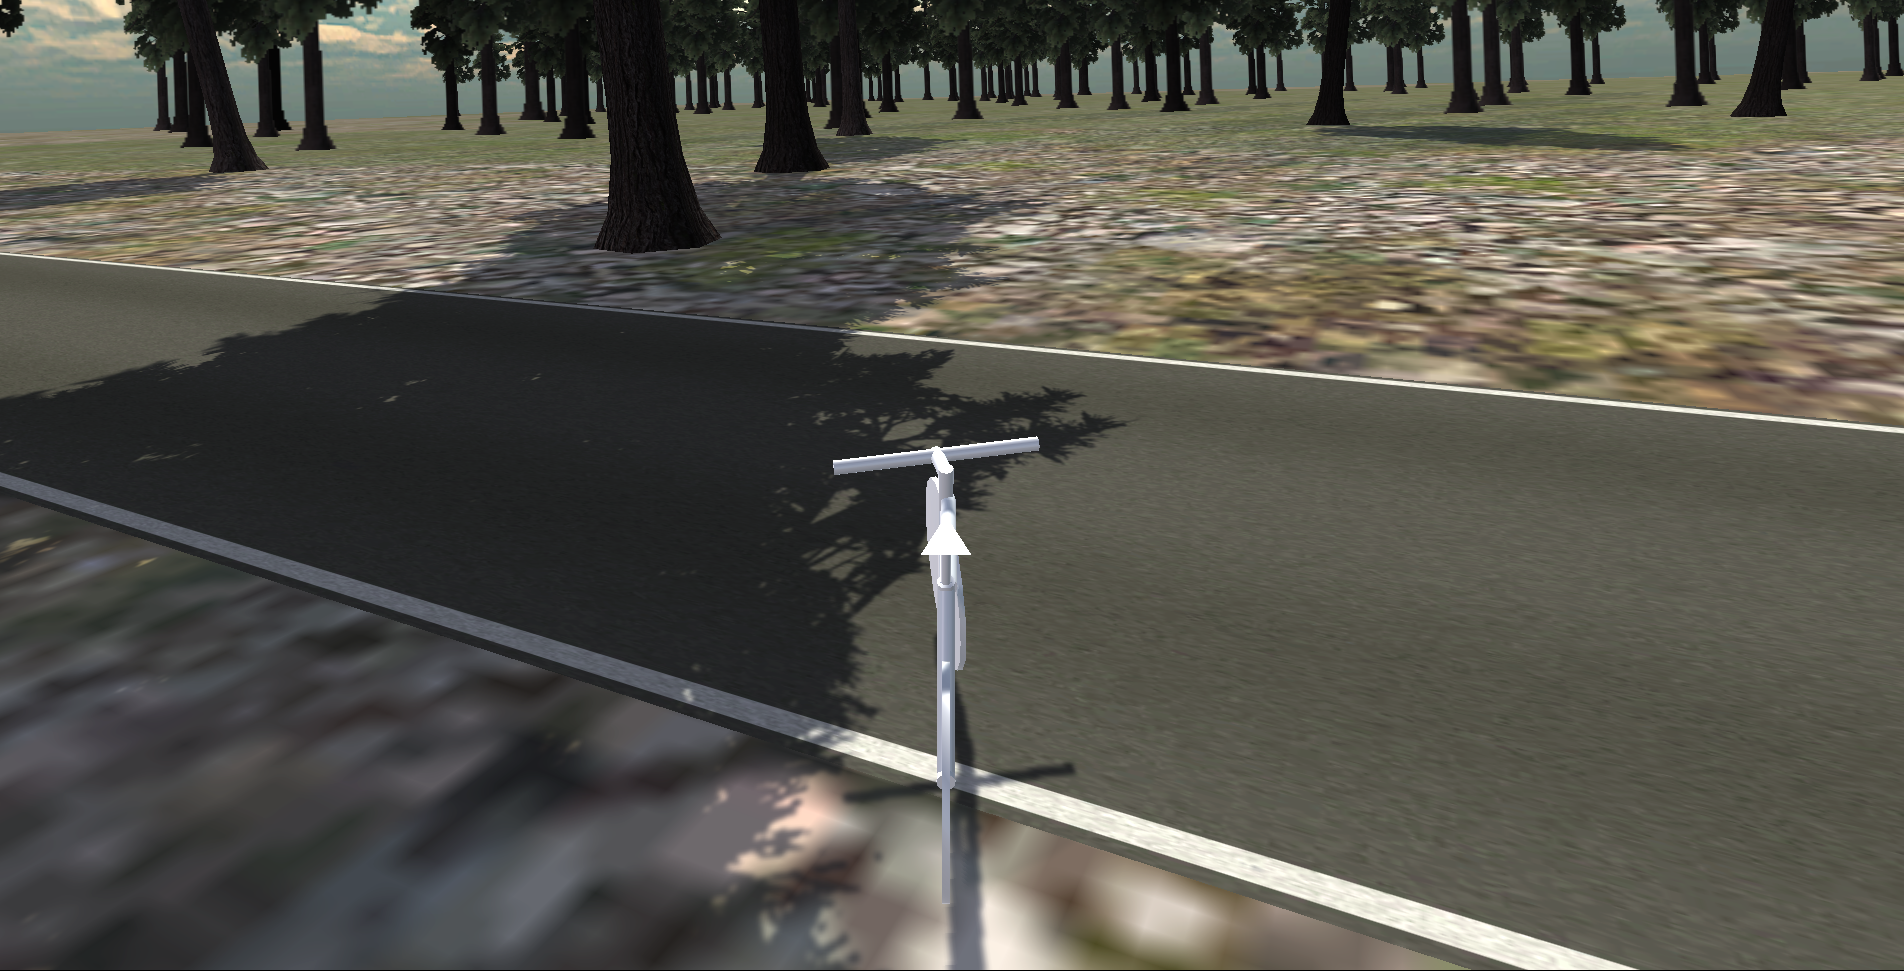
\includegraphics[width=\textwidth]{screenshot_2015-06-27_19-31-15.png}
    \caption{Unity virtual environment with bicycle model}
    \label{fig:unity}
\end{figure}

\subsection{Simulation}
The bicycle dynamics are simulated in \href{https://github.com/oliverlee/bicycle}{C++ code} using the
\href{http://eigen.tuxfamily.org/index.php?title=Main_Page}{Eigen}\cite{eigenweb} template library for linear algebra
operations.
The dynamic equations and kinematic equations are computed in two separate routines and run at two different speeds.

\subsubsection{Dynamics} \label{sec:imp_dyn}
The dynamics loop simulates the \autoref{eq:ss}, and handles communication with the Kollmorgen motor driver.
Measurement of steer angle, estimation of system state, computation of handlebar torque, and transmission of actuator
commands occur within a 1000 Hz loop.
As the bicycle model used in linear, the system is state space model is discretized and reformulated as a difference
equation
\begin{equation}
\begin{aligned}
    \state[k + 1] &= \stateMat_d \state[k] + \inputMat_d \sysInput[k] \\
    \sysOutput[k] &= \outputMat_d \state[k] \label{eq:dtss}
\end{aligned}
\end{equation}
where
\begin{equation}
\begin{aligned}
    \begin{bmatrix} \stateMat_d & \inputMat_d \\ \bm{0} & \bm{I} \end{bmatrix}
        &= \exp(\begin{bmatrix} \stateMat & \inputMat \\ \bm{0} & \bm{0} \end{bmatrix} T_s) \\
    \outputMat_d &= \outputMat \label{eq:c2d}
\end{aligned}
\end{equation}
and $ T_s $ is the sample time.
The matrix exponential is computed using a scaling and squaring with Pad{\'e} approximants algorithm described by
Higham\cite{higham2005}.
While ODE integrators are commonly used, they do not take advantage of the fact that formulation of the equations of
motion are linear and entries in the state and input matrices are constant for a given $ v $.
This formulation allows replaces the typical integration step with a single matrix multiplication, requiring only that
the discrete time state space be computed at each forward speed $ v $.
% states are discretized instead of integrated for efficiency\\
% computation of matrix exponential only once for each foward speed v\\
% ode integration is slower\cite{moler2003} (for computing the matrix exponential)
% note that ode integration for a \textit{single} time step may be slower, \\
% but there is no need to perform all the repeated integration steps as
% we obtain a difference equation. (plus measurement shows it to be faster)

The input torque $ \sysInput[k] $ is estimated using \autoref{eq:handlebar_eom} and a numerical derivative of
acceleration of the handlebar encoder similar to other bicycle simulators\cite{he2005}.

The full state is estimated to obtain the virtual roll angle $ \roll $ and roll rate $ \rollRate $ of the bicycle.
The equations in \autoref{eq:kalman_ss} are discretized in order to use \autoref{eq:c2d}.
The Kalman filter is implemented in standard recursive form with a state prediction step (\textit{a priori})
\begin{equation}
\begin{aligned}
    \stateEst^-[k] &= \stateMat_d \stateEst[k - 1] + \inputMat_d \sysInput[k] \\
    \estimateCov^-[k] &= \stateMat_d \estimateCov[k - 1] \stateMat_d^T + \processCov
\end{aligned}
\end{equation}
followed by a measurement update step (\textit{a posteriori})
\begin{equation}
\begin{aligned}
    \kalmanGain[k] &= \estimateCov^-[k] \outputMat_d^T (\outputMat_d \estimateCov^-[k] \outputMat_d^T + \measCov)^{-1} \\
    \stateEst[k] &= \stateEst^-[k] + \kalmanGain[k] (\meas[k] - \outputMat_d \stateEst^-[k] ) \\
    \estimateCov[k] &= (\bm{I} - \kalmanGain[k] \outputMat_d) \estimateCov^-[k]
\end{aligned}
\end{equation}
where $ \estimateCov $ is the estimate error covariance and ($ ^- $) denotes the term is an \textit{a priori} estimate.
As the model state space matrices described in \autoref{eq:c2d} are parameterized by $ v $, changes in these matrices
are incorporated in the filter prediction and update steps.
Process noise covariance $ \processCov $ and measurement noise covariance $ \measCov $ are taken constant over the
course of the simulation: changes in the model are reflected in state matrices and sensors do not display any
time-dependent behavior.

In selecting the process noise covariance, we consider the system to be an approximation of a constant-velocity
particle\cite{reid2001} as the state vector $ \state $ contains system coordinates and speeds.
We expect a greater order of noise in the system speeds compared to system coordinates and use
\begin{equation}
    \processCov = q \begin{bmatrix}
        T_s & 0 & \frac{1}{2}T_s^2 & 0 \\
        0 & T_s & 0 & \frac{1}{2}T_s^2 \\
        \frac{1}{2}T_s^2 & 0 & \frac{1}{3}T_s^3 & 0 \\
        0 & \frac{1}{2}T_s^2 & 0 & \frac{1}{3}T_s^3 \\
    \end{bmatrix}
\end{equation}
where $ q $ is the uncertainty in $ \steer $ and $ \roll $ due to discretization with sample time $ T_s $.
Measurement noise covariance $ \measCov $ is derived from sensor noise characteristics.

\subsubsection{Kinematics}
The kinematics loop calculates system coordinates required for visualization separately from the dynamics.
Unity is used for visualization and updates at 60 Hz, slower than the haptic update rate.
The ignorable coordinates are divided into two groups and calculated for each visual update.
Rear wheel contact position $ \x $, $ \y $ and yaw angle $ \yaw $ are calculated by integration of \autoref{eq:kineq}
via explicit method Dormand-Prince as implemented in \href{http://www.boost.org/}{Boost}.
While the yaw angle $ \yaw $ is described as linear in terms of system state and it is possible to use a difference
equation as is done in \autoref{sec:imp_dyn}, the three coordinates are computed in the same integration step.
Pitch angle $ \pitch $ is calculated separately using Newton-Raphson and the previous value as an initial guess.
%Built on top of Eigen with separate modules for system model, control, and estimation \\
%2 loops running:
%\begin{itemize}
%    \item simulation loop - ~1000 Hz for sensor acquisition and computation of actuator commands\\
%        timing shows loop duration  $ < 1 $ ms, normally order of us\\
%        no RTOS is used, but profiling shows computation time to be quick enough even with OS interrupts\\
%        so we have enough ``determinism'' in timers
%\begin{itemize}
%    \item states are discretized instead of integrated for efficiency\\
%        computation of matrix exponential only once for each foward speed v\\
%        ode integration is slower\cite{moler2003} (for computing the matrix exponential)
%        note that ode integration for a \textit{single} time step may be slower, \\
%        but there is no need to perform all the repeated integration steps as
%        we obtain a difference equation. (plus measurement shows it to be faster)
%\end{itemize}

\subsection{Hardware interface}
\subsection{Network communication}
As the simulator involves communication between three nodes, data must be serialized and transmitted over a network.
Serialization protocol differs depending on the send/receive nodes due to communication requirements/hardware
advantages?
\subsubsection{Simulation-Visualization communication} \\
Visual coordinates are transmitted between simulation and Unity using the FlatBuffers serialization library.
The protocol allows allows access to serialized data with parsing or unpacking while supporting backwards and forwards
compatibility.
Data is sent through a predefined schema which may evolve over time, although a schema may only add fields if backwards
and forwards compatibility is to be maintained.
Data sent in a scheme may be marked as optional and no data is transmitted if the field is omitted.
\subsubsection{Simulation-Hardware communication} \\
Kollmorgen specified protocol

\section{Hardware design?}

\section{Comparison of data to naturalistic studies}

\begin{table}
    \centering
    \begin{tabular}{|c|l|}
        \hline
        symbol & description \\
        \hline
        $ \x $ & rear wheel contact point in x-direction \\
        $ \y $ & rear wheel contact point in y-direction \\
        $ \pitch $ & rear frame pitch angle \\
        $ \yaw $ & rear frame yaw angle \\
        $ \roll $ & rear wheel roll angle \\
        $ \steer $ & relative rotation between front and rear frame about steer-axis\\
        \hline
    \end{tabular}
    \caption{Whipple coordinates}
    \label{tab:coordinates}
\end{table}

\begin{table}
    \centering
    \begin{tabular}{|c|l|}
        \hline
        symbol & description \\
        \hline
        $ w $ & wheelbase \\
        $ c $ & trail \\
        $ \lambda $ & steer axis tilt \\
        $ r_r $ & rear wheel radius \\
        $ r_f $ & front wheel radius \\
        \hline
    \end{tabular}
    \caption{Meijaard-Whipple parameters}
    \label{tab:parameters}
\end{table}

\section{Conclusions}
\section{Future work}
\begin{itemize}
    \item Feedback terrain data from virtual environment to affect steering feel
    \item Implement realistic pedaling
\end{itemize}

\section{Acknowledgments}
We gratefully acknowledge the European Commission for their support of the Marie Curie Initial Training Network (ITN)
project Nr. 608092 MOTORIST (Motorcycle Rider Integrated Safety), www.motorist-ptw.eu.

\bibliography{references.bib}
\bibliographystyle{plain}
\end{document}

Note from Arend:
In this work we address the need for haptic feedback in the balancing task in bicycling. For that we use an experimental
bicycle simulator setup which has been described in Recuero and Schwab 2013. The system, which is shown in
Fig~\ref{fig1}, consists of a stationary bicycle on which one can pedal and steer. The visual feedback is by means of a
real time animation on a flat computer screen, with either a first or third person view. The steering assembly has
torque feedback from the computer model. In this bicycle simulator the rider interacts with a virtual environment,
receiving realistic handlebar torque from a bicycle model, which runs in the computer simulation model. The lateral
dynamics of the bicycle are governed by the linearized equations of motion for lean and
steer~\cite{meijaard2007linearized} as implemented in the computer model. The state of the handlebar, lean angle and
lean angle rate, are measured and together with the computer generated lean angle and its time derivatives used to
estimate handlebar haptic feedback torque $T_m$. The steer dynamics is governed by the real handlebar system. Stability
of the haptic system for any kind of human contribution, e.g., tight grasp or sudden release, must be guaranteed. In so
doing, one can resort to place a ``virtual coupling'' between the haptic device and the virtual environment that acts as
a mechanical filter~\cite{adams1999stable}. The bicycle haptic interface, as developed here, shows a impedance
casuality, i.e., forces are transmitted to the rider, whereas the input of the virtual environment is the handlebar
state. Uncertainties in the measurement of steering angle and its rate may lead, depending on the physical model
utilized, to unrealistic fed back torque or excessive phase lag~\cite{katzourakis2009design}. The set of sample rates of
sensors and the model is another key factor in the haptic system. It must be high enough to keep a pleasant refreshing
rate of the simulator visualization and results in natural and smooth feeling in rider's limbs.
